\subsection{Модуль Telegram-бот}

Telegram-бот представляет в СКУД средство пользовательского управления работой
системы. Бот связует две части -- серверную и клиентскую с помощью серверов
Telegram (см. Рис 26).

\begin{figure}[h!]
  \centering
  \setlength{\fboxsep}{5pt}
  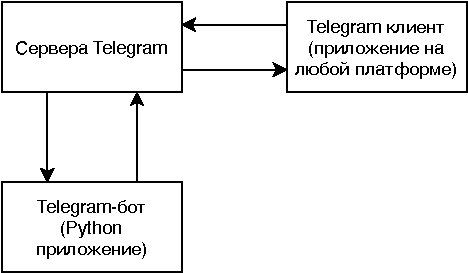
\includegraphics[width=0.6\textwidth]{data-visualisation/telegram-bot-arch}
  \vspace*{6pt}
  \caption{Структура связи Telegram-бота и клиента}\label{fig:image-processing}
\end{figure}

Функционал бота определяет:

\begin{itemize*}
\item беспрерывное обновление данных;
\item построение пользовательских меню;
\item составление диалога с пользователем;
\end{itemize*}

\subsubsection{Получение и отправка данных Telegram-ботом}

В дипломном проекте использовалась прораммная "обёртка" над Telegram Bot API -- библиотека pyTelegramBotAPI, выполняющая API запросы функцией Python. 

Библиотека инкапсулирует все вызовы API в один класс -- TeleBot. Для запуска бота требуется создать экземляр класса Telebot (см. Рисунок 27)

\begin{lstlisting}
from telebot import TeleBot

# TOKEN - уникальный код владельца бота, можно сгенерировать в 
# Father Bot, родительском боте. 
bot = TeleBot(TOKEN)
\end{lstlisting}

Для получения новых сообщений, требуется создать специальные функции
с параметрами ожидаемых сообщений (тип, условие и т.п.):

\begin{lstlisting}
# Функция для обработки сообщения с командой "Статус" 
@bot.message_handler(func=lambda message: message.text == "Статус")
def cmd_status(msg):
  # do something

# Функция для обработки сообщения, содержащего
# изображение
@bot.message_handler(content_types=["photo"])
def photo_msg(msg):
  # do something
\end{lstlisting}

Отправка новых сообщений выполняется функциями из класса TeleBot:

\begin{lstlisting}
# Отправка сообщения
# CHAT_ID - идентификатор чата, RESPONSE - сообщение
bot.send_message(CHAT_ID, RESPONSE)

# Отправка изображения
bot.send_photo(CHAT_ID, photo)
\end{lstlisting}
